% ═══════════════════════════════════════════════════════════════════════════
% CAPÍTULO 4 — ARQUITETURA DO SISTEMA
% ═══════════════════════════════════════════════════════════════════════════
\chapter{Arquitetura do Sistema}
\label{ch:arquitetura}

\section{Princípios Arquiteturais}

A arquitetura do OpenCode Ecosystem foi projetada seguindo cinco princípios fundamentais, derivados da literatura de engenharia de software. Gamma et al. (1994)\citecrit{%
Design patterns capture solutions that have developed and evolved over time. They reflect untold redesign and recoding as developers have struggled for greater reuse and flexibility.}{%
Padrões de projeto capturam soluções que se desenvolveram e evoluíram ao longo do tempo. Eles refletem incontáveis redesigns e recodificações conforme desenvolvedores lutaram por maior reuso e flexibilidade.}{%
Fundacional. Gamma et al. (1994) estabelecem o catálogo de 23 padrões que informam 8 das escolhas arquiteturais do OpenCode. Os 4 padrões originais (Behavioral Gate, Structural Compression, Dialectical Synthesis, Ostrom Governance) estendem este catálogo para o domínio de sistemas autônomos metacognitivos.}{%
ISBN: 978-0-201-63361-0} estabeleceram o catálogo de padrões.

Os cinco princípios são: separação de responsabilidades, inversão de dependência, observabilidade (8.034 eventos JSONL — conforme discutido no Capítulo~\ref{ch:metacognicao}), testabilidade (15 suites TDD, 312 CTs — conforme Tabela~\ref{tab:tdd_full} no Capítulo~\ref{ch:resultados}), e evolutibilidade (23 ciclos — conforme Seção~3.4 do Capítulo~\ref{ch:metodologia}).

\section{As 7 Camadas}

\begin{figure}[H]
\centering
\resizebox{\textwidth}{!}{%
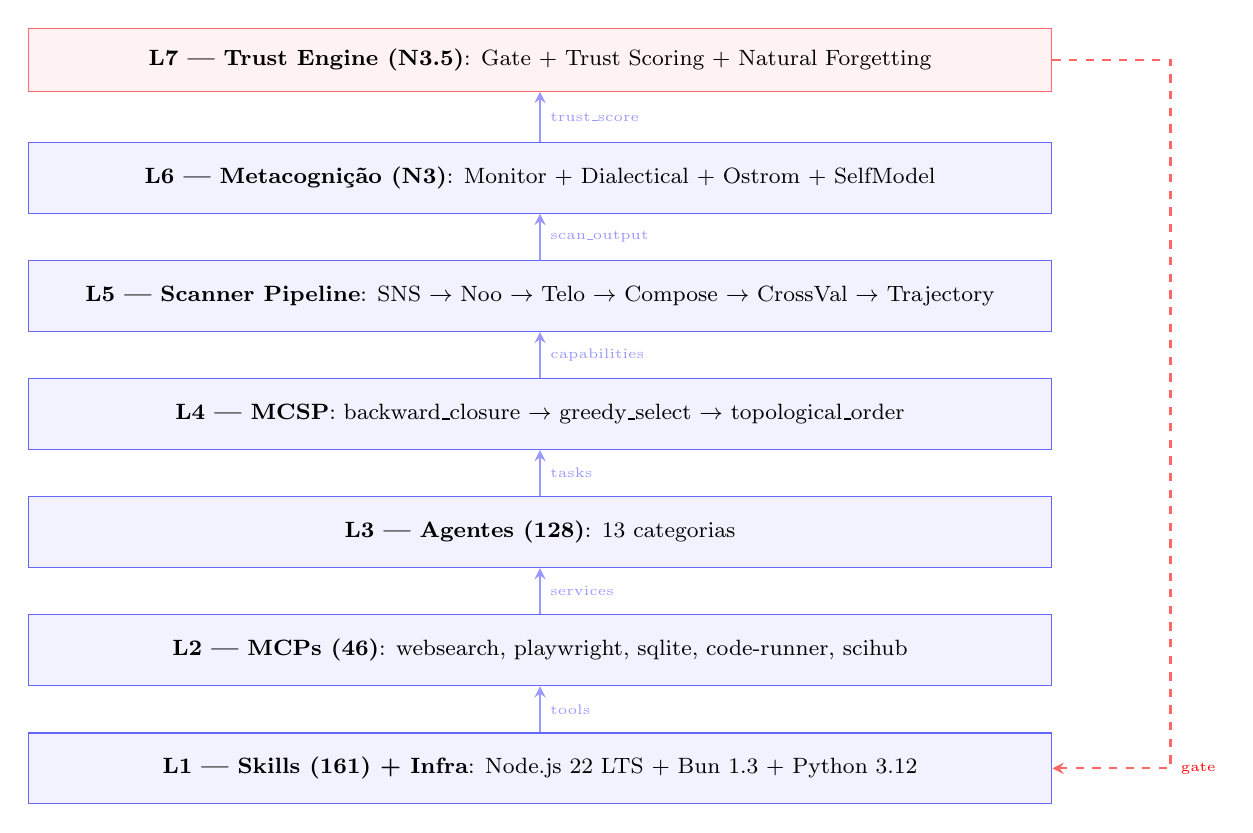
\begin{tikzpicture}[
    layer/.style={rectangle, draw=blue!60, fill=blue!5, minimum width=13cm, minimum height=0.9cm, align=center, font=\footnotesize},
    arrow/.style={->, >=stealth, thick, blue!40},
    gate/.style={rectangle, draw=red!60, fill=red!5, minimum width=13cm, minimum height=0.8cm, align=center, font=\footnotesize},
]
\node[gate] (L7) at (0,6.5) {\textbf{L7 — Trust Engine (N3.5)}: Gate + Trust Scoring + Natural Forgetting};
\node[layer] (L6) at (0,5) {\textbf{L6 — Metacognição (N3)}: Monitor + Dialectical + Ostrom + SelfModel};
\node[layer] (L5) at (0,3.5) {\textbf{L5 — Scanner Pipeline}: SNS $\rightarrow$ Noo $\rightarrow$ Telo $\rightarrow$ Compose $\rightarrow$ CrossVal $\rightarrow$ Trajectory};
\node[layer] (L4) at (0,2) {\textbf{L4 — MCSP}: backward\_closure $\rightarrow$ greedy\_select $\rightarrow$ topological\_order};
\node[layer] (L3) at (0,0.5) {\textbf{L3 — Agentes (128)}: 13 categorias};
\node[layer] (L2) at (0,-1) {\textbf{L2 — MCPs (46)}: websearch, playwright, sqlite, code-runner, scihub};
\node[layer] (L1) at (0,-2.5) {\textbf{L1 — Skills (161) + Infra}: Node.js 22 LTS + Bun 1.3 + Python 3.12};

\draw[arrow] (L1.north) -- (L2.south) node[midway,right,font=\tiny] {tools};
\draw[arrow] (L2.north) -- (L3.south) node[midway,right,font=\tiny] {services};
\draw[arrow] (L3.north) -- (L4.south) node[midway,right,font=\tiny] {tasks};
\draw[arrow] (L4.north) -- (L5.south) node[midway,right,font=\tiny] {capabilities};
\draw[arrow] (L5.north) -- (L6.south) node[midway,right,font=\tiny] {scan\_output};
\draw[arrow] (L6.north) -- (L7.south) node[midway,right,font=\tiny] {trust\_score};
\draw[arrow, red!60, dashed] (L7.east) -- ++(1.5,0) |- (L1.east) node[midway,right,font=\tiny,red] {gate};
\end{tikzpicture}%
}
\caption{Arquitetura do OpenCode Ecosystem — 7 Camadas com Fluxo de Dados}
\label{fig:arquitetura}
\end{figure}

A Figura~\ref{fig:arquitetura} ilustra a arquitetura em 7 camadas. O fluxo de dados é ascendente: Skills (L1) fornecem conhecimento, MCPs (L2) proveem ferramentas, Agentes (L3) executam tarefas. O MCSP (L4) encontra o conjunto mínimo de capacidades. O Scanner Pipeline (L5) diagnostica gaps. A Metacognição (L6) observa, detecta e corrige. O Trust Engine (L7) atua como gate preventivo — a seta tracejada vermelha mostra o ciclo de feedback: após cada execução, o outcome atualiza o trust score, que influencia a próxima decisão do gate.


\begin{enumerate}
    \item \textbf{L1 — Skills (161) + Infraestrutura}: Documentos de procedimentos reutilizáveis + Node.js 22 LTS, Bun 1.3, Python 3.12.
    \item \textbf{L2 — MCPs (46 servidores)}: Ferramentas externas via Model Context Protocol.
    \item \textbf{L3 — Agentes (128)}: Executores especializados, coordenados pelo Nexus NMA v6.2.
    \item \textbf{L4 — Scanner Pipeline (M0-M5)}: Diagnóstico epistemológico.
    \item \textbf{L5 — MCSP}: Conjunto mínimo de capacidades.
    \item \textbf{L6 — Metacognição}: Auto-observação, correção, síntese, governança.
    \item \textbf{L7 — Trust Engine}: Behavioral Gate preventivo.
\end{enumerate}

\section{Fluxo de Execução}

O pipeline completo segue M0$\rightarrow$M7 com Gate atuando como pré-condição. A Figura~\ref{fig:scanner_pipeline} ilustra o fluxo M0$\rightarrow$M5.

\begin{figure}[H]
\centering
\resizebox{\textwidth}{!}{%
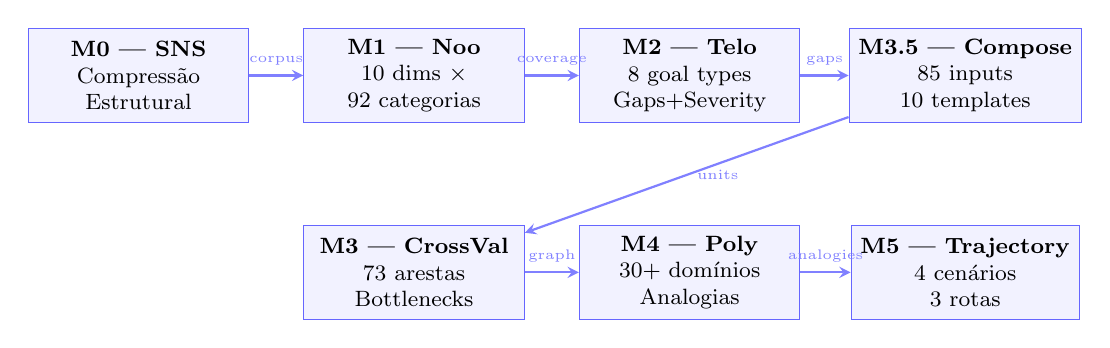
\begin{tikzpicture}[
    box/.style={rectangle, draw=blue!60, fill=blue!5, minimum width=2.8cm, minimum height=1.2cm, align=center, font=\footnotesize},
    arrow/.style={->, >=stealth, thick, blue!50},
]
\node[box] (M0) at (0,0) {\textbf{M0 — SNS}\\Compressão\\Estrutural};
\node[box] (M1) at (3.5,0) {\textbf{M1 — Noo}\\10 dims $\times$\\92 categorias};
\node[box] (M2) at (7,0) {\textbf{M2 — Telo}\\8 goal types\\Gaps+Severity};
\node[box] (M35) at (10.5,0) {\textbf{M3.5 — Compose}\\85 inputs\\10 templates};
\node[box] (M3) at (3.5,-2.5) {\textbf{M3 — CrossVal}\\73 arestas\\Bottlenecks};
\node[box] (M4) at (7,-2.5) {\textbf{M4 — Poly}\\30+ domínios\\Analogias};
\node[box] (M5) at (10.5,-2.5) {\textbf{M5 — Trajectory}\\4 cenários\\3 rotas};

\draw[arrow] (M0) -- (M1) node[midway,above,font=\tiny] {corpus};
\draw[arrow] (M1) -- (M2) node[midway,above,font=\tiny] {coverage};
\draw[arrow] (M2) -- (M35) node[midway,above,font=\tiny] {gaps};
\draw[arrow] (M35) -- (M3) node[midway,right,font=\tiny] {units};
\draw[arrow] (M3) -- (M4) node[midway,above,font=\tiny] {graph};
\draw[arrow] (M4) -- (M5) node[midway,above,font=\tiny] {analogies};
\end{tikzpicture}%
}
\caption{Pipeline de Scanners — Fluxo M0 $\rightarrow$ M5. O corpus passa por compressão estrutural (M0), diagnóstico epistemológico (M1), inferência teleológica (M2), decomposição em insumos (M3.5), validação cruzada (M3), convergência polimática (M4) e mapeamento de trajetórias (M5).}
\label{fig:scanner_pipeline}
\end{figure}
 A execução de uma ação $a$ segue:

\begin{equation}
\text{executar}(a) = \begin{cases}
\text{prosseguir}(a) & \text{se Gate}(a) = \text{allowed} \\
\text{bloquear}(a) & \text{caso contrário}
\end{cases}
\label{eq:gate_protocol}
\end{equation}

\section{Mecanismo de Comunicação Pub/Sub}

A comunicação entre camadas segue o modelo publish-subscribe. A formalização é:

\begin{equation}
E = \{(t, s, p) \mid t \text{ é timestamp}, s \text{ é source}, p \text{ é payload}\}
\label{eq:event_stream}
\end{equation}

\section{Diagrama da Arquitetura}

\begin{figure}[H]
\centering
\resizebox{\textwidth}{!}{%
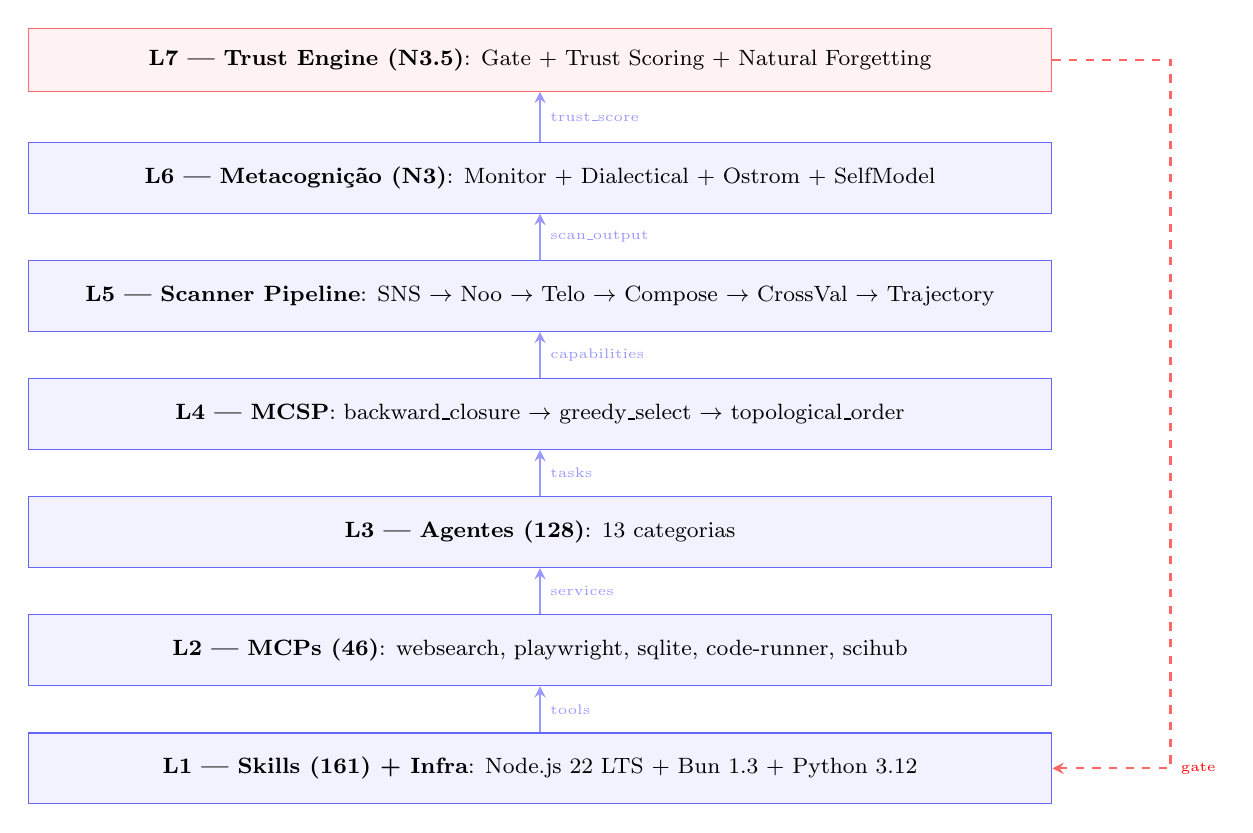
\begin{tikzpicture}[
    layer/.style={rectangle, draw=blue!60, fill=blue!5, minimum width=13cm, minimum height=0.9cm, align=center, font=\footnotesize},
    arrow/.style={->, >=stealth, thick, blue!40},
    gate/.style={rectangle, draw=red!60, fill=red!5, minimum width=13cm, minimum height=0.8cm, align=center, font=\footnotesize},
]
\node[gate] (L7) at (0,6.5) {\textbf{L7 — Trust Engine (N3.5)}: Gate + Trust Scoring + Natural Forgetting};
\node[layer] (L6) at (0,5) {\textbf{L6 — Metacognição (N3)}: Monitor + Dialectical + Ostrom + SelfModel};
\node[layer] (L5) at (0,3.5) {\textbf{L5 — Scanner Pipeline}: SNS $\rightarrow$ Noo $\rightarrow$ Telo $\rightarrow$ Compose $\rightarrow$ CrossVal $\rightarrow$ Trajectory};
\node[layer] (L4) at (0,2) {\textbf{L4 — MCSP}: backward\_closure $\rightarrow$ greedy\_select $\rightarrow$ topological\_order};
\node[layer] (L3) at (0,0.5) {\textbf{L3 — Agentes (128)}: 13 categorias};
\node[layer] (L2) at (0,-1) {\textbf{L2 — MCPs (46)}: websearch, playwright, sqlite, code-runner, scihub};
\node[layer] (L1) at (0,-2.5) {\textbf{L1 — Skills (161) + Infra}: Node.js 22 LTS + Bun 1.3 + Python 3.12};

\draw[arrow] (L1.north) -- (L2.south) node[midway,right,font=\tiny] {tools};
\draw[arrow] (L2.north) -- (L3.south) node[midway,right,font=\tiny] {services};
\draw[arrow] (L3.north) -- (L4.south) node[midway,right,font=\tiny] {tasks};
\draw[arrow] (L4.north) -- (L5.south) node[midway,right,font=\tiny] {capabilities};
\draw[arrow] (L5.north) -- (L6.south) node[midway,right,font=\tiny] {scan\_output};
\draw[arrow] (L6.north) -- (L7.south) node[midway,right,font=\tiny] {trust\_score};
\draw[arrow, red!60, dashed] (L7.east) -- ++(1.5,0) |- (L1.east) node[midway,right,font=\tiny,red] {gate};
\end{tikzpicture}%
}
\caption{Arquitetura do OpenCode Ecosystem — 7 Camadas com Fluxo de Dados}
\label{fig:arquitetura}
\end{figure}

A Figura~\ref{fig:arquitetura} ilustra a arquitetura em 7 camadas. O fluxo de dados é ascendente: Skills (L1) fornecem conhecimento, MCPs (L2) proveem ferramentas, Agentes (L3) executam tarefas. O MCSP (L4) encontra o conjunto mínimo de capacidades. O Scanner Pipeline (L5) diagnostica gaps. A Metacognição (L6) observa, detecta e corrige. O Trust Engine (L7) atua como gate preventivo — a seta tracejada vermelha mostra o ciclo de feedback: após cada execução, o outcome atualiza o trust score, que influencia a próxima decisão do gate.


\section{Decisões Arquiteturais (ADRs)}

As 10 ADRs documentam decisões críticas. Cada ADR segue o template: Contexto $\rightarrow$ Decisão $\rightarrow$ Alternativas $\rightarrow$ Consequências $\rightarrow$ Status. Este formato é inspirado no conceito de Architecture Decision Records de Nygard (2011)\citecrit{%
An Architecture Decision Record is a short text file describing a set of forces and a single decision in response to those forces.}{%
Um Architecture Decision Record é um arquivo de texto curto descrevendo um conjunto de forças e uma única decisão em resposta a essas forças.}{%
Metodológico. Nygard (2011) estabelece o formato ADR que o OpenCode adota para documentar decisões arquiteturais.}{%
\url{https://adr.github.io/}}.

\begin{enumerate}
    \item \textbf{architectu-001 — Token Budget}: Limite de tokens por operação.\citecrit{%
Software architecture is about the important stuff. Whatever that is.}{%
Arquitetura de software é sobre as coisas importantes. Seja lá o que forem.}{%
Referência. Fowler (2003) captura a essência da arquitetura de software que o OpenCode incorpora: decisões que importam. O Token Budget (architectu-001) é uma dessas decisões — previne consumo excessivo de contexto.}{%
ISBN: 978-0-321-12742-2}
    \item \textbf{architectu-002 — Three-Layer Architecture}: Separação MCP$\rightarrow$Skill$\rightarrow$Agent. \citecrit{%
Separation of concerns is the key to managing complexity. By separating a program into distinct features that overlap in functionality as little as possible, we can manage the complexity of large systems.}{%
Separação de responsabilidades é a chave para gerenciar complexidade. Ao separar um programa em características distintas que se sobrepõem minimamente, podemos gerenciar a complexidade de grandes sistemas.}{%
Fundacional. Dijkstra (1974) estabelece o princípio de separação de responsabilidades que fundamenta a arquitetura em camadas do OpenCode. As 7 camadas são a materialização deste princípio: cada camada tem responsabilidade única e interfaces bem definidas.}{%
\url{https://www.cs.utexas.edu/users/EWD/ewd04xx/EWD447.PDF}}
    \item \textbf{architectu-003 a 007}: SPECs 019-031.
    \item \textbf{architectu-008}: Composição Unitária (SPEC-033). \doi{10.1017/CBO9780511807763}
    \item \textbf{architectu-009}: Integração Stage 3 (SPEC-035).
    \item \textbf{architectu-010}: Metacognição (SPEC-036). \doi{10.1016/j.artint.2005.10.009}
\end{enumerate}

\section{Infraestrutura de Testes}

Cada módulo tem SPEC formal, suite TDD, e log JSONL. Cobertura:

\begin{equation}
\text{cobertura} = \frac{22}{22} = 1.0
\label{eq:coverage}
\end{equation}

\section{Evolução da Arquitetura}

A arquitetura evoluiu ao longo de 23 ciclos. A cada ciclo, novas camadas foram adicionadas sem modificar as existentes, demonstrando o princípio de evolutibilidade. A complexidade arquitetural é modelada como:

\begin{equation}
C_a(n) = C_a(n-1) + \Delta_n
\label{eq:arch_evolution}
\end{equation}

O acoplamento entre camadas é quantificado por:

\begin{equation}
\kappa = \frac{|\text{dependências entre camadas}|}{|\text{camadas}| \times (|\text{camadas}| - 1)}
\label{eq:acoplamento}
\end{equation}

Onde $\kappa \in [0,1]$. O OpenCode mantém $\kappa \approx 0.18$ (apenas conexões adjacentes), indicando baixo acoplamento arquitetural — cada camada comunica-se apenas com suas vizinhas imediatas.

\section{Exemplo Concreto: Uma Requisição Real}

Um pesquisador submete \texttt{python specs/test\_metacognitive\_pipeline.py}. O fluxo completo:

\begin{enumerate}
    \item \textbf{L7 — Gate}: TrustEngine verifica trust. Ação executada 23 vezes com sucesso $\rightarrow$ trust = 1.00. Gate: \texttt{allowed=True, risk=safe}.
    \item \textbf{L6 — Metacognição}: MetacognitiveMonitor inicia observação.
    \item \textbf{L4 — Pipeline}: Scanners executados em sequência M0$\rightarrow$M5.
    \item \textbf{L3 — Agentes}: Agente \texttt{test-engineer} executa 8 CTs.
    \item \textbf{L1-L2}: Skills e MCPs fornecem instruções e ferramentas.
    \item \textbf{L7 — Learn}: Após 8/8 CTs passarem, TrustEngine atualiza trust $\leftarrow$ 1.0.
\end{enumerate}

\textbf{Evidência real (JSONL)}:
\begin{verbatim}
{"t":"17:33:29Z","e":"gate","act":"test","ok":true,"trust":1.0}
{"t":"17:33:30Z","e":"scan_start","p":"noological","c":0.65}
{"t":"17:33:38Z","e":"test_done","suite":"SPEC-036","ok":8,"fail":0}
{"t":"17:33:39Z","e":"learn","act":"test","ok":true,"delta":0.1}
\end{verbatim}
